subsubsection{Estensione C: Errore di Salvataggio della Controproposta}

In alcune circostanze, l’invio della controproposta può fallire a causa di problemi di connessione o di errori del server.  
Il sistema gestisce questa eventualità mostrando all’utente un chiaro feedback visivo sull’esito dell’operazione.

\subsubsection{Gestione dell’Errore e Comunicazione all’Utente}
Dopo aver cliccato su \textbf{“Invia controproposta”}, viene mostrato un breve stato di caricamento.  
Se il salvataggio non va a buon fine, compare un pop-up di allerta che informa l’agente dell’errore e della mancata registrazione della controproposta.

L’utente può chiudere l’allerta e tentare nuovamente l’operazione una volta ristabilita la connessione.  
Questo comportamento supporta la \textbf{recuperabilità dall’errore}, assicurando che l’utente non perda il lavoro svolto e possa riprovare senza dover reinserire tutti i dati.

\begin{figure}[H]
	\centering
	\begin{tikzpicture}[node distance=1.5cm and 1cm, auto]
		% Nodo per immagine 2 con didascalia sotto, posizionato a destra di img1
		\node (img1) {
			\begin{tabular}{c}
				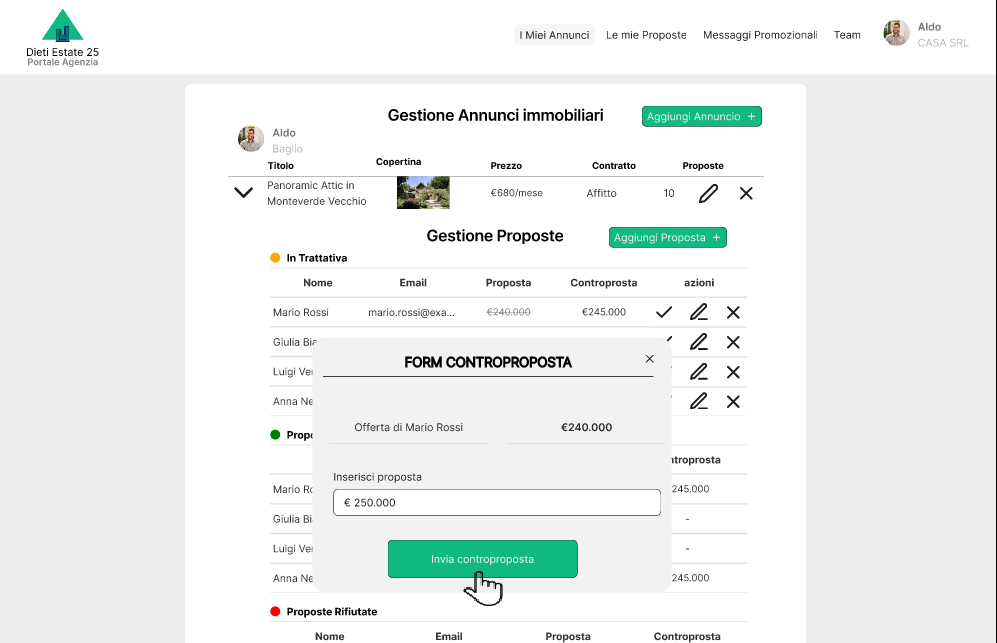
\includegraphics[width=0.7\textwidth]{Immagini/Mockup/controproposte/scenario principale/ClickInviaControproposta.png} \\
				Cockburn: step 7.C/8.C
			\end{tabular}
		};
		
		% Nodo per immagine 3 con didascalia sotto, posizionato sotto img2
		\node (img2) [below=of img1] {
			\begin{tabular}{c}
				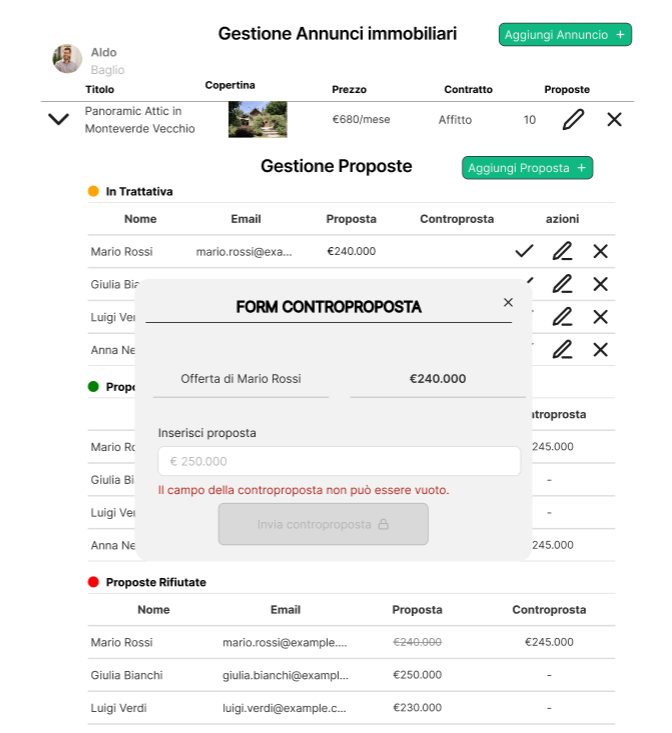
\includegraphics[width=0.7\textwidth]{Immagini/Mockup/controproposte/Extensions C/MessaggioDiErrore.png} \\
				Cockburn: step 9.C
			\end{tabular}
		};
		
		% Disegna le frecce
		\draw[->, thick] (img1) -- (img2);
		
	\end{tikzpicture}
	\caption{Mockup: Extension C della tabella di Cockburn del caso d'uso: Fare una controproposta a un'offerta.}
	\label{fig:tikz_flow}
\end{figure}

\newpage


